\documentclass[conference,a4paper]{IEEEtran}
\IEEEoverridecommandlockouts

\usepackage[T1]{fontenc}
\usepackage{cite}
\usepackage{amsmath,amssymb,amsfonts}
\usepackage{graphicx}
\usepackage{booktabs}
\usepackage{multirow}
\usepackage{makecell}
\usepackage{array}
\usepackage{xcolor}
\usepackage{url}
\usepackage[hidelinks,pdfusetitle]{hyperref}
\hypersetup{
  pdftitle={Hallucination Space Projection for Whisper: Reproduction, an Affine Variant, and a Threshold Baseline},
  pdfauthor={Nongmaithem Hans, Ravikant Sharma},
  pdfkeywords={speech recognition, Whisper, hallucination, activation editing, voice activity, reproducibility}
}
\def\UrlBreaks{\do\/\do-}

% Notation
\newcommand{\pns}{p_{\mathrm{ns}}}
\newcommand{\pnsbase}{p_{\mathrm{ns}}^{\mathrm{base}}}
\newcommand{\hall}{\mathrm{hall}}
\newcommand{\empt}{\mathrm{empty}}
\newcommand{\repo}{\url{https://github.com/h4444n55555/Reducing-Hallucinations-in-Whispr}}

\begin{document}

\title{Hallucination Space Projection for Whisper:\\
Reproduction, an Affine Variant,\\ and a Threshold Baseline}

\author{%
\IEEEauthorblockN{Nongmaithem Hans}
\IEEEauthorblockA{\textit{Indian Institute of Technology Ropar}\\
Rupnagar, Punjab, India\\
Entry no.\ 2024AIB1011}
\and
\IEEEauthorblockN{Ravikant Sharma}
\IEEEauthorblockA{\textit{Indian Institute of Technology Ropar}\\
Rupnagar, Punjab, India\\
Entry no.\ 2024AIB1013}
}

\maketitle

\begin{abstract}
Whisper often outputs fluent text such as ``thank you'' for audio that contains no speech. A recent paper proposes a training-free fix: remove a low-rank ``hallucination subspace'' from one decoder layer, only for clips that Whisper already suspects are non-speech. It reports that mean non-speech hallucination rate (HR) falls from 31.31\% to 3.74\% across three model sizes. We re-implement the method and reproduce it on Whisper small with real data. Our tuned setting lowers held-out HR from 28.41\% to 1.27\%, and the paper's own setting gives 3.14\% against the published 3.07\%. However, plain Whisper with a lower no-speech threshold, chosen on the same development data by the same rule, reaches 0.87\% HR with lower word error rate (5.93\% vs.\ 6.58\%) and equal false rejections (1.35\%). At equal HR, the projection rejects significantly more speech (McNemar $p = 0.024$). At the paper's operating point, the edit acts on speech exactly like a threshold. We explain why projecting the last layer fails and test an affine variant that moves states toward the empty-class mean instead of zero. It removes the last-layer failure, but its selected setting generalises poorly (held-out HR 12.61\% against 4.0\% on development data), and at equal HR it again rejects more speech than a threshold (7 vs.\ 0 utterances, $p = 0.016$). Because Whisper's decoder is causal, restricting the edit to the SOT position cannot change any rejection, so it cannot close this gap. Code, results and an interactive dashboard are available at \repo.
\end{abstract}

\begin{IEEEkeywords}
speech recognition, Whisper, hallucination, activation editing, voice activity, reproducibility
\end{IEEEkeywords}

% ---------------------------------------------------------------------------
\section{Introduction}

Large weakly supervised speech recognisers such as Whisper~\cite{radford2023whisper} transcribe non-speech audio (silence, noise, music) into plausible text: ``thank you'', ``you'', subtitle endings, or a repeated syllable. Because the text is fluent, downstream systems can take it for real speech. Whisper has no separate voice-activity detector. At the first decoding step its decoder predicts a special no-speech token, and the probability of that token, $\pns$, decides rejection: a segment is dropped when $\pns > \tau = 0.6$. A hallucination occurs when the decoder gives that token a low probability on non-speech audio.

Abbasihafshejani and Jadliwala~\cite{abbasi2026hsp} propose to remove a low-rank subspace from one decoder layer's hidden states, estimated once from non-speech clips that do and do not hallucinate, and to apply the edit only when the unedited $\pns$ already exceeds a small gate $\gamma$. Without training, they report large HR reductions on three model sizes, at a cost of 0.33 to 4.39 WER points and 0.41\% to 9.97\% falsely rejected utterances on LibriSpeech.

This report makes four contributions:
\begin{itemize}
\item A re-implementation in a single notebook and an end-to-end reproduction on Whisper small, including the paper's own operating point.
\item A threshold baseline that the paper omits: plain Whisper with $\tau$ chosen on development data by the paper's own selection rule, compared clip by clip with paired significance tests.
\item An analysis of what the gate and the edit actually do, and of why editing the last decoder layer fails.
\item An affine variant of the projection, which the last-layer analysis motivates.
\end{itemize}
Fig.~\ref{fig:arch} gives an overview of the full experimental pipeline.

\begin{figure*}[!t]
\centering
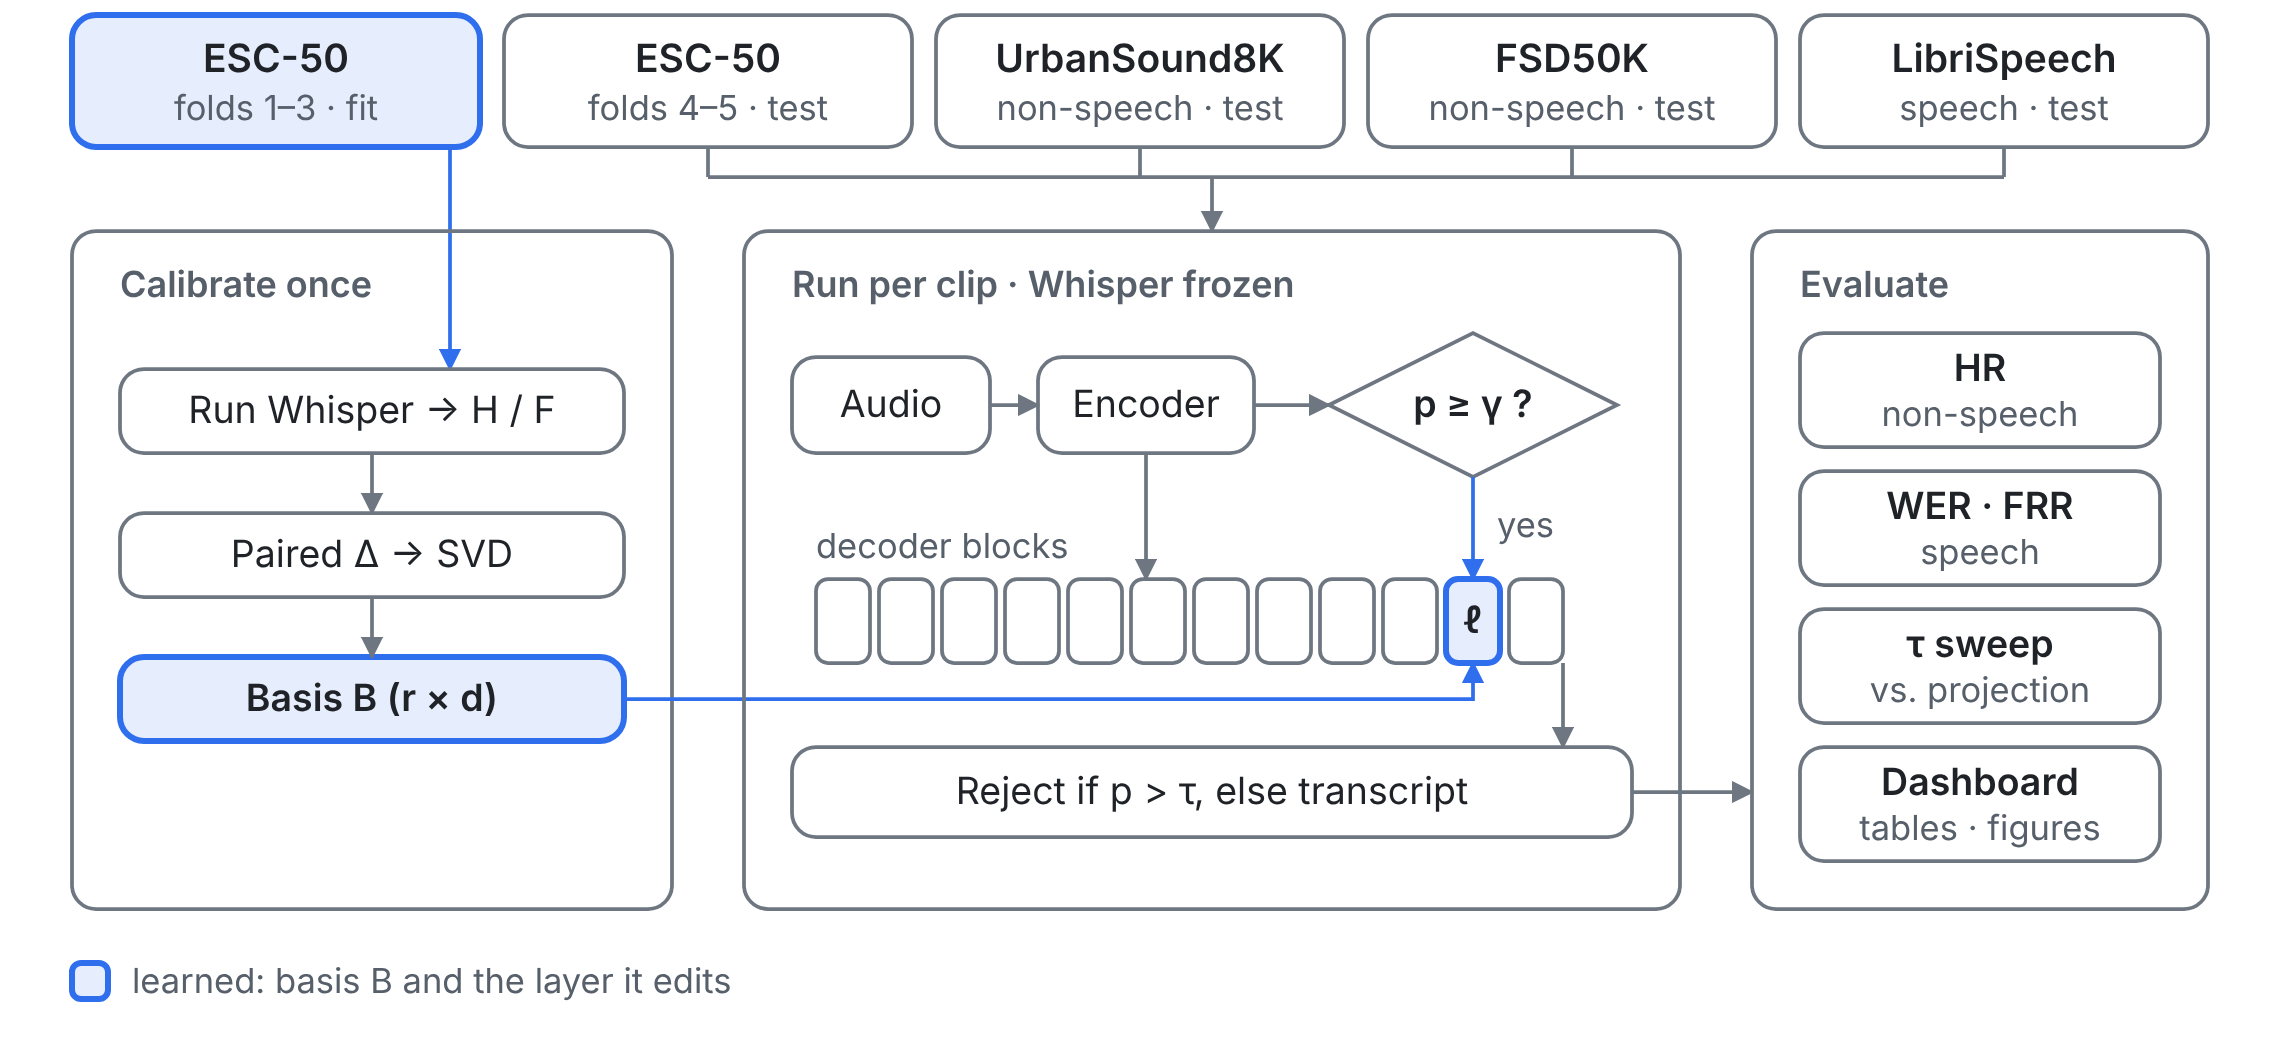
\includegraphics[width=0.92\textwidth]{fig_architecture_c.png}
\caption{Overview of the experimental pipeline. The basis $B$ (rank $r$, model width $d$) is fitted once on ESC-50 folds 1--3 and applied at a single decoder layer $\ell$ of frozen Whisper; the edit is applied only when the gate $\pns \ge \gamma$ opens. Held-out evaluation uses ESC-50 folds 4--5, UrbanSound8K and FSD50K (non-speech) and LibriSpeech (speech). Shaded boxes are the learned components.}
\label{fig:arch}
\end{figure*}

% ---------------------------------------------------------------------------
\section{Background and Related Work}

Earlier fixes act at other points of the pipeline. External voice-activity detection, as in WhisperX~\cite{bain2023whisperx}, filters the input audio but needs a second model and segmentation. Bag of Hallucinations~\cite{baranski2025boh} removes frequent hallucinated phrases from the output, but misses phrases not in its list. Calm-Whisper~\cite{wang2025calm} fine-tunes three decoder heads, which needs training data. Lowering $\tau$ acts on the output score and needs nothing at all, but~\cite{abbasi2026hsp} reports that it ``changes little'' in the range it tests (0.5 to 0.9).

The projection follows activation-editing work on language models, which removes an estimated hallucination subspace from hidden states. Linear concept erasure is known to be optimal when it is affine~\cite{belrose2023leace}, which motivates our affine variant.

% ---------------------------------------------------------------------------
\section{Method}


\subsection{Calibration sets}
Whisper is run on non-speech calibration clips (ESC-50~\cite{piczak2015esc} folds 1--3, 1,200 clips). Each clip goes into one of two groups by its own outcome at $\tau = 0.6$: $H$, the clips with a non-empty transcript, and $F$, the clips left empty. For each clip the decoder state at layer $\ell$ is kept; following the point where $\pns$ is read, we take the state at the start-of-transcript (SOT) position.

\subsection{Hallucination subspace}
\label{sec:subspace}
Rows of $H$ and $F$ are paired and subtracted, so acoustic factors shared by all non-speech audio cancel. The top $r$ right singular vectors of the difference matrix form the basis $B_{\ell,r}$, with orthonormal rows:
\begin{equation*}
\Delta_\ell =
\begin{bmatrix}
h^{\hall}_1 - h^{\empt}_1\\ \vdots \\ h^{\hall}_n - h^{\empt}_n
\end{bmatrix}
= U\Sigma V^{\top}, \qquad B_{\ell,r} = V^{\top}_{1:r},
\end{equation*}
with $n = \min(N_h, N_f)$ pairs taken in file order.

\subsection{Projection and the affine variant}
A forward hook on block $\ell$ edits every hidden state $h$, at every position, with strength $\alpha$:
\begin{equation}
\tilde{h} = h - \alpha\,(hB^{\top})\,B .
\label{eq:proj}
\end{equation}
With $\alpha = 1$ the component of $h$ inside $\operatorname{span}(B)$ is set to zero. Our affine variant instead moves that component to the value of the correctly-empty class, $c$ = mean of the $F$ states at layer $\ell$:
\begin{equation}
\tilde{h} = h - \alpha\,\big((h - c)B^{\top}\big)\,B .
\label{eq:affine}
\end{equation}
Eq.~\eqref{eq:affine} changes only the target of the edit; $B$, the gate and the selection procedure are unchanged.

\subsection{Gate and rejection}
A first, unedited forward pass gives $\pnsbase$. The clip is decoded with the hook only if $\pnsbase \ge \gamma$, and the result is rejected if its own $\pns > \tau$ (Fig.~\ref{fig:arch}, centre). The always-on variant skips the gate. Since every rejected clip has passed the gate, and both decisions read Whisper's own $\pns$, the natural control is plain Whisper with a lower $\tau$.

% ---------------------------------------------------------------------------
\section{Experimental Setup}

\subsection{Data}
Calibration uses all 1,200 clips of ESC-50 folds 1--3 (256 hallucinate, 944 stay empty; HR 21.3\%). Development data for parameter selection are 400 of these clips and 200 utterances of LibriSpeech~\cite{panayotov2015librispeech} dev-clean, as in~\cite{abbasi2026hsp}. The development non-speech clips are therefore also used to fit $B$ and $c$; Sec.~\ref{sec:robust} measures how much this matters. Held-out sets are listed in Table~\ref{tab:data}; to fit a laptop GPU we use seeded random subsets of the larger sets.

\begin{table}[!t]
\centering
\caption{Held-out evaluation sets}
\label{tab:data}
\begin{tabular}{@{}llrr@{}}
\toprule
Set & Type & Used & Full \\
\midrule
ESC-50 folds 4--5~\cite{piczak2015esc} & non-speech & 800 & 800 \\
UrbanSound8K~\cite{salamon2014urbansound} & non-speech & 2,000 & 8,732 \\
FSD50K eval~\cite{fonseca2022fsd50k} & non-speech & 2,000 & 8,598 \\
LibriSpeech test-clean & speech & 1,000 & 2,620 \\
LibriSpeech test-other & speech & 1,000 & 2,939 \\
\bottomrule
\end{tabular}\\[3pt]
\parbox{0.95\columnwidth}{\footnotesize FSD50K: clips labelled \emph{Speech} or \emph{Human\_voice} removed. Removing music labels as well, as the text of~\cite{abbasi2026hsp} states, leaves only 6,729 clips; the paper's count of 8,621 suggests music was kept, so we keep it.}
\end{table}

\subsection{Metrics}
Hallucination rate (HR) is the share of non-speech clips with any text left after rejection. Word error rate (WER) is computed on LibriSpeech after Whisper's English normaliser; a rejected utterance counts as all words deleted. False-rejection rate (FRR) is the share of speech utterances rejected. We report the mean HR over the three non-speech sets and the mean WER and FRR over the two speech sets.

\subsection{Implementation}
Everything runs in one notebook on the official \texttt{openai-whisper} package: greedy decoding, English forced, no timestamps, audio padded or cut to 30\,s. Rejection uses $\pns$ alone, as in Algorithm~1 of~\cite{abbasi2026hsp}. Each clip is decoded once, with or without the hook: $\pnsbase$ is fixed by the first decoder step, so this equals the paper's ``decode, then re-decode if gated'' and halves the cost. Weights are cast to fp16 once, decodes are shared between methods, clips that will be rejected are not decoded, and long loops checkpoint and resume. Sanity tests on a tiny random Whisper check before every run that the hook removes exactly the intended component, that the affine edit lands on $c$, and that the one-pass $\pns$ equals what \texttt{whisper.decode} reports. Every per-clip output, including the unfiltered text and $\pns$, is saved, so other thresholds can be scored without decoding again. The full run took about three hours on an RTX~3050 6\,GB laptop GPU (fp16, seed 0, batch 16): about one for Eq.~\eqref{eq:proj} and the baselines, and two for the affine variant.

\subsection{Parameter selection}
We follow~\cite[Sec.~5.1]{abbasi2026hsp}. Stage~1 sweeps layer $\ell \in \{1,\dots,12\}$ and rank $r \in \{1,2,4,8\}$ with always-on projection and $\alpha = 1$. Stage~2 fixes $\ell$ and $r$ and sweeps $\alpha \in \{0.25, 0.5, 0.75, 1\}$ and $\gamma \in \{0.03, 0.05, 0.10, 0.15\}$ with the gate. In both stages we take the lowest dev HR among settings whose dev WER is within 0.5 points of plain Whisper (ties: lowest WER). The same procedure is run separately for Eq.~\eqref{eq:proj} and Eq.~\eqref{eq:affine}. For the threshold baseline the same rule picks $\tau$ from a grid of step 0.01. Table~\ref{tab:op} lists the selected operating points.

\begin{table}[!t]
\centering
\caption{Operating points}
\label{tab:op}
\begin{tabular}{@{}lcccc@{}}
\toprule
Setting & $\ell$ & $r$ & $\alpha$ & $\gamma$ \\
\midrule
Paper~\cite{abbasi2026hsp}, small & 10 & 1 & 1.0 & 0.15 \\
Ours, Eq.~\eqref{eq:proj} & 11 & 8 & 1.0 & 0.05 \\
Ours, affine Eq.~\eqref{eq:affine} & 10 & 2 & 1.0 & 0.05 \\
\bottomrule
\end{tabular}\\[3pt]
\parbox{0.95\columnwidth}{\footnotesize Plain-Whisper threshold chosen on dev with the same rule: $\tau = 0.17$ ($\tau = 0.14$--$0.17$ tie at dev HR 0\% and unchanged dev WER; we take the largest).}
\end{table}

% ---------------------------------------------------------------------------
\section{Results}

\begin{figure*}[!t]
\centering
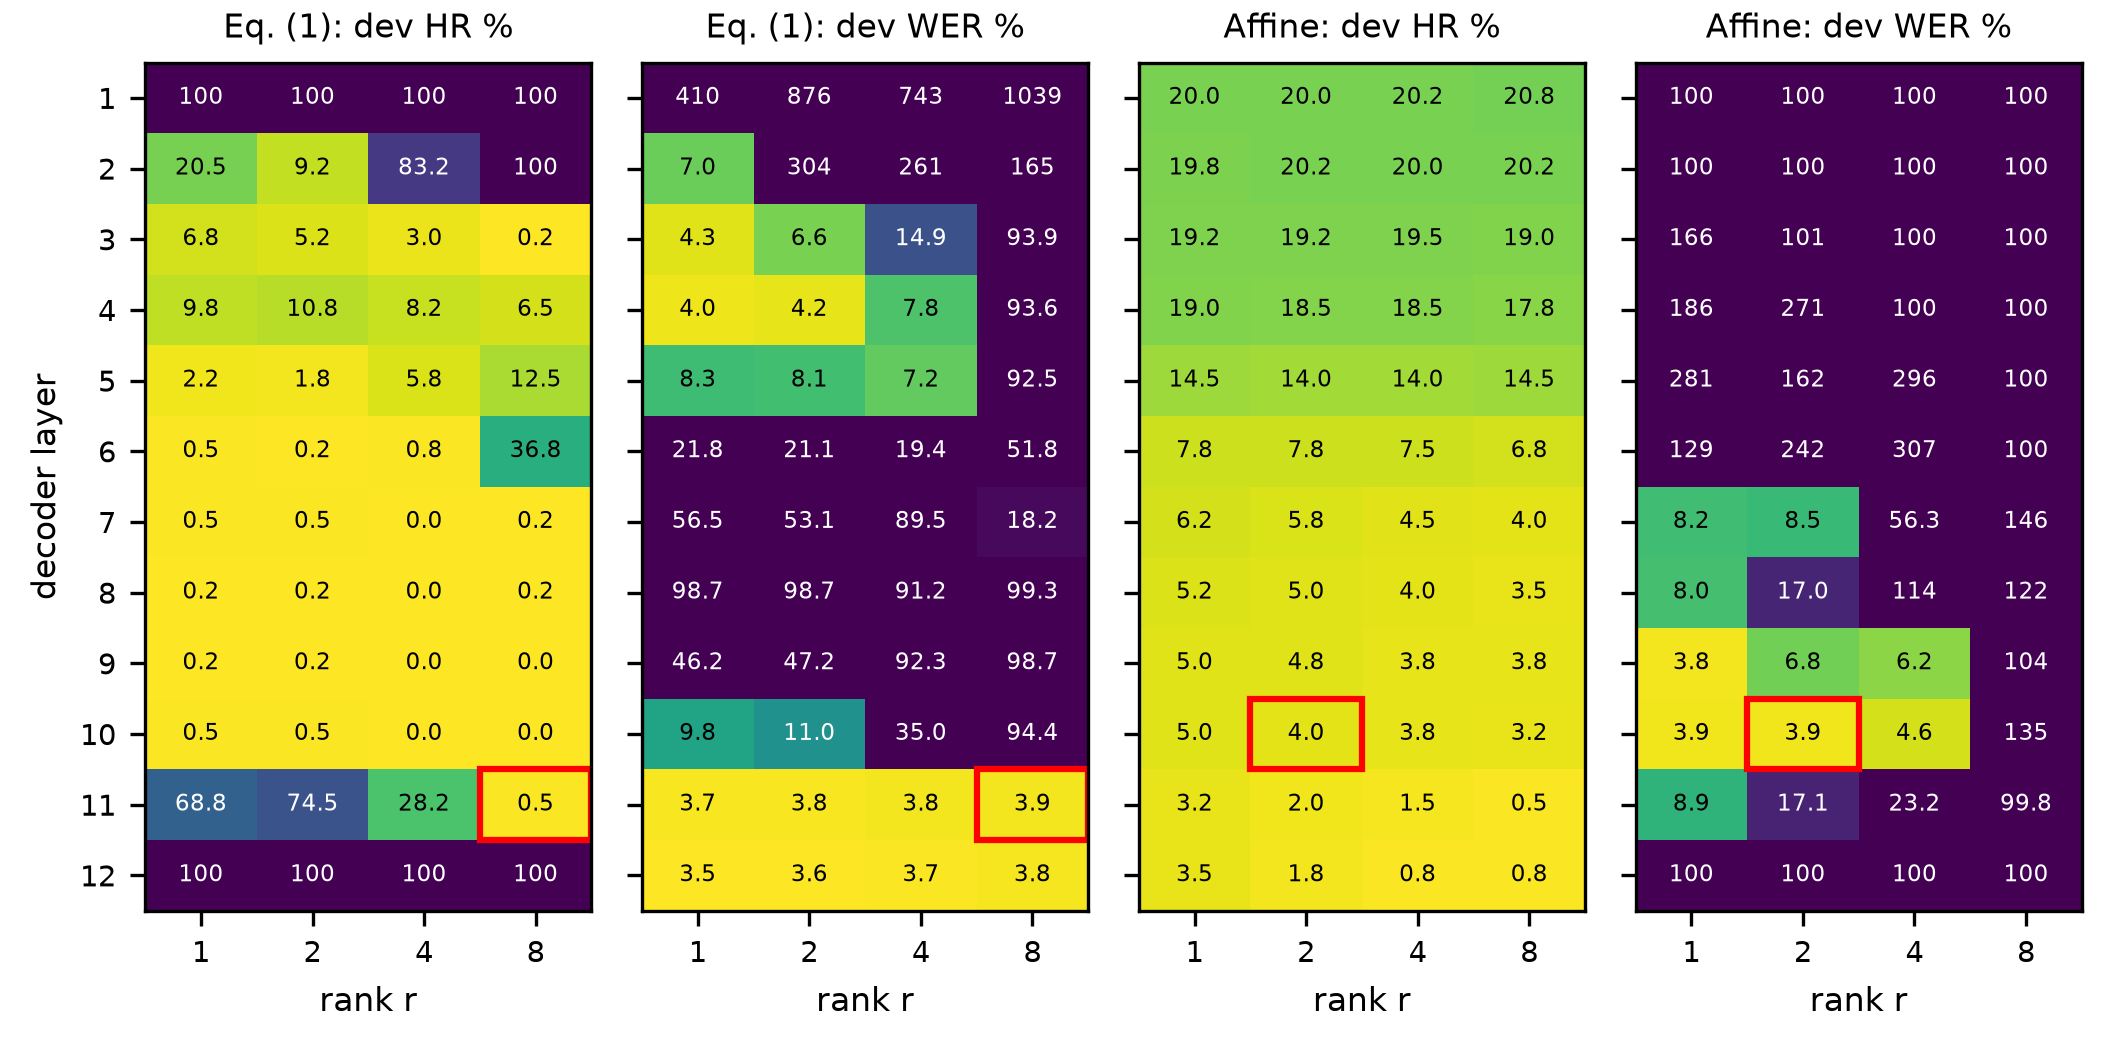
\includegraphics[width=\textwidth]{fig_stage1_c.png}
\caption{Stage-1 sweep on development data (always-on, $\alpha = 1$). Left pair: Eq.~\eqref{eq:proj}; right pair: affine Eq.~\eqref{eq:affine}. Red boxes mark the selected settings; WER colour is capped at 19\%. Plain Whisper: HR 20.0\%, WER 3.59\%.}
\label{fig:stage1}
\end{figure*}

\subsection{Parameter selection}
For Eq.~\eqref{eq:proj} the usable region is narrow (Fig.~\ref{fig:stage1}). Nine of 48 settings keep dev WER within 0.5 points: layer 4 at rank 1 and every rank at layers 11 and 12. Of these, only layer 11 at rank 8 also has low HR (0.5\%). Middle layers (6--10) remove hallucinations but reject 6.5\% to 98.5\% of dev speech; the paper's own point, layer 10 at rank 1, gives dev WER 9.8\% and FRR 6.5\% here. Layers 1 and 12 fail at every rank, with HR 100\%. In stage~2, HR falls steadily with $\alpha$ (14.75\%, 7.25\%, 3.0\%, 0.5\% for $\alpha = 0.25$ to 1), while $\gamma$ changes neither HR nor FRR on dev, because 200 clean utterances rarely reach $\pns \ge 0.03$.

The affine sweep looks different (Fig.~\ref{fig:stage1}, right pair; Fig.~\ref{fig:layers}). Dev FRR stays at or below 0.5\% at layers 1--11, so the edit no longer rejects speech, and HR falls smoothly with depth instead of jumping between 0\% and 100\%. Dev WER, however, is 100\% or more for most settings: the transcripts are destroyed without being rejected (Sec.~\ref{sec:affine}). Only three settings stay within 0.5 points (layer 9 at rank 1, layer 10 at ranks 1 and 2), and the rule selects layer 10, rank 2 (dev HR 4.0\%, WER 3.89\%). In stage~2 HR again falls with $\alpha$ (16.75\%, 11.75\%, 8.75\%, 4.0\%), and $\gamma$ again leaves HR unchanged.

\begin{table*}[!t]
\centering
\caption{Held-out results on Whisper small (\%). HR: lower is better on non-speech; WER and FRR: lower is better on speech}
\label{tab:main}
\setlength{\tabcolsep}{5pt}
\begin{tabular}{@{}l rrr r rr rr rr@{}}
\toprule
& \multicolumn{4}{c}{Non-speech HR $\downarrow$} & \multicolumn{2}{c}{WER $\downarrow$} & \multicolumn{2}{c}{FRR $\downarrow$} & \multicolumn{2}{c}{Speech avg.} \\
\cmidrule(lr){2-5}\cmidrule(lr){6-7}\cmidrule(lr){8-9}\cmidrule(l){10-11}
Method & ESC-50 & US8K & FSD50K & Avg & clean & other & clean & other & WER & FRR \\
\midrule
Plain Whisper, $\tau = 0.6$ & 26.12 & 14.50 & 44.60 & 28.41 & 3.31 & 7.63 & 0.0 & 0.0 & 5.47 & 0.00 \\
Bag of Hallucinations~\cite{baranski2025boh} & 13.75 & 8.90 & 18.45 & 13.70 & 3.31 & 7.63 & 0.0 & 0.0 & 5.47 & 0.00 \\
\midrule
Always-on, Eq.~\eqref{eq:proj}, $\ell$11 $r$8 & 0.50 & 1.50 & 1.75 & 1.25 & 3.37 & 10.25 & 0.2 & 3.3 & 6.81 & 1.75 \\
Gated, Eq.~\eqref{eq:proj}, $\ell$11 $r$8 & 0.50 & 1.50 & 1.80 & 1.27 & 3.50 & 9.66 & 0.2 & 2.5 & 6.58 & 1.35 \\
Always-on, paper point & 1.38 & 0.55 & 7.10 & 3.01 & 8.20 & 19.49 & 6.7 & 14.7 & 13.84 & 10.70 \\
Gated, paper point & 1.38 & 0.65 & 7.40 & 3.14 & 3.91 & 8.41 & 1.4 & 2.4 & 6.16 & 1.90 \\
Gate only (reject if $\pns \ge 0.05$) & 0.00 & 0.00 & 0.20 & 0.07 & 13.07 & 20.68 & 14.9 & 20.7 & 16.87 & 17.80 \\
\midrule
Always-on, affine, $\ell$10 $r$2 & 8.38 & 6.60 & 22.85 & 12.61 & 2.92 & 7.87 & 0.1 & 0.6 & 5.40 & 0.35 \\
Gated, affine, $\ell$10 $r$2 & 8.38 & 6.60 & 22.85 & 12.61 & 3.32 & 8.03 & 0.1 & 0.6 & 5.68 & 0.35 \\
Gated, affine, $\ell$11 $r$8 & 1.00 & 1.30 & 1.80 & 1.37 & 13.03 & 20.65 & 0.9 & 5.4 & 16.84 & 3.15 \\
Gated, affine, paper point & 9.25 & 7.00 & 24.25 & 13.50 & 3.31 & 7.65 & 0.1 & 0.1 & 5.48 & 0.10 \\
\midrule
\textbf{Plain Whisper, $\boldsymbol{\tau = 0.17}$ (dev)} & 0.25 & 0.30 & 2.05 & \textbf{0.87} & 3.72 & 8.14 & 1.2 & 1.5 & \textbf{5.93} & \textbf{1.35} \\
\bottomrule
\end{tabular}\\[3pt]
\parbox{\textwidth}{\footnotesize Published values for comparison~\cite{abbasi2026hsp}, small, gated: HR 1.53 / 0.84 / 6.84; WER 4.37 / 9.13; FRR 0.41 / 2.58. Plain: HR 23.50 / 12.33 / 21.35; WER 4.04 / 8.38. US8K: UrbanSound8K.}
\end{table*}

\subsection{Held-out results and agreement with the paper}
Gated projection at the paper's operating point reproduces the published HR closely (1.38 / 0.65 / 7.40 vs.\ 1.53 / 0.84 / 6.84; Table~\ref{tab:main}). The WER increase over plain Whisper is similar ($+0.60$ / $+0.78$ points vs.\ $+0.33$ / $+0.75$), and so is test-other FRR (2.4\% vs.\ 2.58\%); test-clean FRR is higher (1.4\% vs.\ 0.41\%). Always-on projection at the paper's point costs much more speech than reported (WER 8.20 / 19.49 vs.\ 4.51 / 11.48). Plain Whisper's FSD50K HR is 44.6\% here against 21.35\% in~\cite{abbasi2026hsp}; the paper prints 21.35\% for both small and large-v3, and our value is close to its medium value (41.95\%). Music does not explain the gap: plain Whisper hallucinates on 38.8\% of our FSD50K clips with a music label and on 46.2\% of the rest. Our tuned Eq.~\eqref{eq:proj} setting lowers mean HR to 1.27\%, below the paper's point (3.14\%), at slightly higher WER (6.58\% vs.\ 6.16\%) and lower FRR (1.35\% vs.\ 1.90\%).

\subsection{A tuned threshold matches or beats the projection}
On development data the threshold alone already beats the projection: $\tau = 0.17$ gives dev HR 0.00\% with dev WER unchanged (3.59\%), against 0.50\% and 3.57\% for the selected Eq.~\eqref{eq:proj} setting. On held-out data $\tau = 0.17$ gives HR 0.87\% vs.\ 1.27\%, WER 5.93\% vs.\ 6.58\%, and the same FRR (Table~\ref{tab:main}); it is lower or equal on all three. Within the dev tie the choice matters little: $\tau = 0.15$ gives HR 0.71\%, WER 6.18\%, FRR 2.0\%. No projection setting lies below or to the left of the threshold curve (Fig.~\ref{fig:tradeoff}). The no-speech probability already separates speech from non-speech almost perfectly (AUROC 0.9991; Fig.~\ref{fig:pns}), and projection does not improve that (0.9986 gated, 0.9983 always-on). The two distributions overlap only between about 0.1 and 0.3, which is where a dev-tuned $\tau$ falls.

\begin{figure}[!t]
\centering
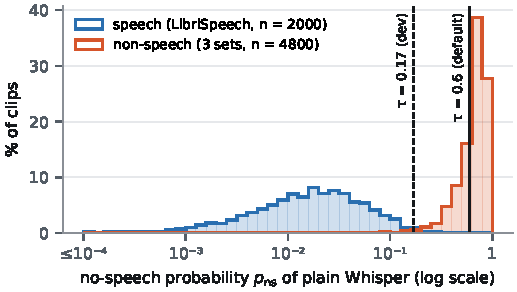
\includegraphics[width=\columnwidth]{fig_pns.pdf}
\caption{Distribution of plain Whisper's no-speech probability on the held-out sets (speech: LibriSpeech test-clean and test-other; non-speech: ESC-50 folds 4--5, UrbanSound8K, FSD50K). Vertical lines: default and dev-tuned thresholds.}
\label{fig:pns}
\end{figure}

\begin{figure}[!t]
\centering
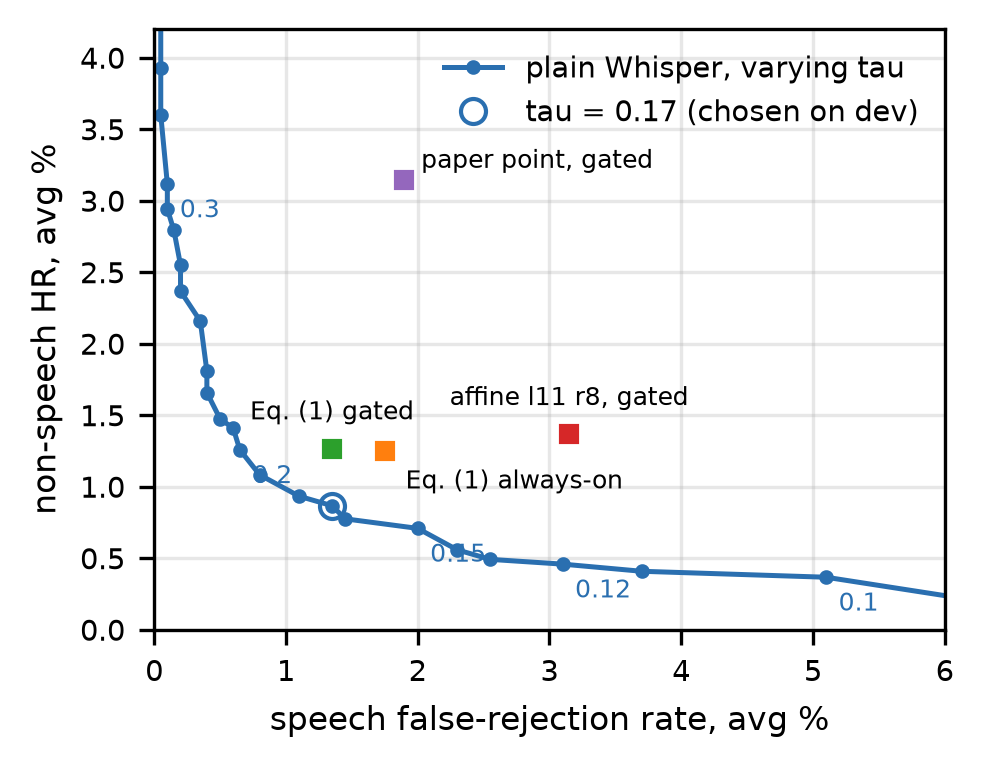
\includegraphics[width=\columnwidth]{fig_tradeoff.png}
\caption{Held-out trade-off. Line: plain Whisper as $\tau$ varies (no projection); the ring marks $\tau$ chosen on dev. Squares: projection settings. Points off the axes are listed in Table~\ref{tab:main}.}
\label{fig:tradeoff}
\end{figure}

\subsection{Paired significance tests}
Both methods run on the same clips, so we compare them clip by clip: an exact McNemar test~\cite{mcnemar1947} on the clips that only one method gets wrong, and a paired bootstrap over utterances (2,000 resamples) for WER. Table~\ref{tab:paired} compares each projection with plain Whisper at the $\tau$ that gives the same held-out HR.

\begin{table*}[!t]
\centering
\caption{Paired tests at equal held-out HR: each projection against plain Whisper at the threshold $\tau$ that matches its HR}
\label{tab:paired}
\begin{tabular}{@{}l c rrr rrr c@{}}
\toprule
& & \multicolumn{3}{c}{Speech rejected (utterances)} & \multicolumn{3}{c}{Non-speech hallucinated (clips)} & \\
\cmidrule(lr){3-5}\cmidrule(lr){6-8}
Projection & Matched $\tau$ & Only proj. & Only $\tau$ & $p$ & Only proj. & Only $\tau$ & $p$ & $\Delta$WER, points [95\% CI] \\
\midrule
Gated Eq.~\eqref{eq:proj}, $\ell$11 $r$8 & 0.20 & 24 & 10 & 0.024 & 45 & 46 & 1.0 & $+0.95$ [0.40, 1.56] \\
Gated, paper point & 0.30 & 36 & 0 & $3\cdot10^{-11}$ & 91 & 91 & 1.0 & $+0.68$ [0.40, 0.99] \\
Gated affine Eq.~\eqref{eq:affine}, $\ell$10 $r$2 & 0.46 & 7 & 0 & 0.016 & 192 & 169 & 0.25 & $+0.21$ [0.06, 0.41] \\
\bottomrule
\end{tabular}\\[3pt]
\parbox{\textwidth}{\footnotesize Only proj.\,/\,only $\tau$: clips that only one of the two methods gets wrong; $p$: exact McNemar test. $\Delta$WER: average over test-clean and test-other of projection minus threshold, with paired-bootstrap 95\% interval (2,000 resamples).}
\end{table*}

At equal HR every projection rejects significantly more speech than the threshold, and its WER is significantly higher, by 0.95, 0.68 and 0.21 points. On non-speech no projection differs significantly from the threshold that matches its HR.

\subsection{What the gate and the edit do}
At the paper's operating point ($\gamma = 0.15$) the gate opens for 14 of 1,000 test-clean utterances and 26 of 1,000 test-other utterances, and the projection then rejects all 14 test-clean and 24 of the 26 test-other ones. On speech, the method is therefore the threshold ``reject if $\pns \ge 0.15$''. Plain Whisper at $\tau = 0.15$ gives the same speech numbers (WER 3.91 / 8.45, FRR 1.4 / 2.6, against 3.91 / 8.41 and 1.4 / 2.4) with lower HR (0.71\% vs.\ 3.14\%).

Our setting differs. With $\gamma = 0.05$ the gate opens for 99.9\% of non-speech clips, so on non-speech the gated method is effectively always-on. On speech it opens for 149 test-clean utterances (2 rejected) and 207 test-other utterances (25 rejected), which is why rejecting every gated clip (gate only, Table~\ref{tab:main}) is a poor control. The edit does not harm the transcripts it keeps: on the same projected and accepted utterances, WER goes from 4.55\% to 4.65\% (test-clean, $n = 147$) and from 10.80\% to 10.49\% (test-other, $n = 182$); for always-on, from 3.30\% to 3.18\% and from 7.73\% to 7.76\%. The whole WER cost is rejection, and the rejected utterances are short (at the paper's point 9.1 words on test-clean and 7.4 on test-other, against averages of 20.2 and 18.2).

\subsection{Why the last layer fails}
\label{sec:lastlayer}
The state after the last block goes directly to the final LayerNorm and output embedding, so $\pns$ can be recomputed from the saved calibration states, with and without the edit (the recomputation matches the saved values within 0.004). Because calibration labels are defined by $\pns$, the direction separating $H$ from $F$ is largely the no-speech read-out: the coordinate on the first basis vector correlates with $\log \pns$ at $-0.73$. That coordinate is far from zero in both groups ($-79.6$ for hallucinated clips, $-91.6$ for empty ones). Eq.~\eqref{eq:proj} sets it to zero, moving every clip 80 to 90 units in the direction that lowers $\pns$: the share of calibration clips with $\pns > 0.6$ drops from 78.7\% to 0\%, at every rank. Nothing is rejected any more, which is the 100\% HR of Fig.~\ref{fig:stage1}. Eq.~\eqref{eq:proj} is therefore not a neutral removal; it moves states to the origin of the subspace, far from where either class lies. The affine edit (Eq.~\eqref{eq:affine}) moves the coordinate to the $F$ mean instead, and does what the method intends: the share of calibration clips with $\pns > 0.6$ rises from 78.7\% to 95.2\% at rank 1 and to 99.4\% at rank 8. At layer 12 dev HR is now 3.5\% to 0.75\% rather than 100\%. It is still not usable there, because every speech utterance is either rejected (dev FRR 57.5\% at rank 1, 5.5\% at rank 8) or decoded into garbage.

\begin{figure*}[!t]
\centering
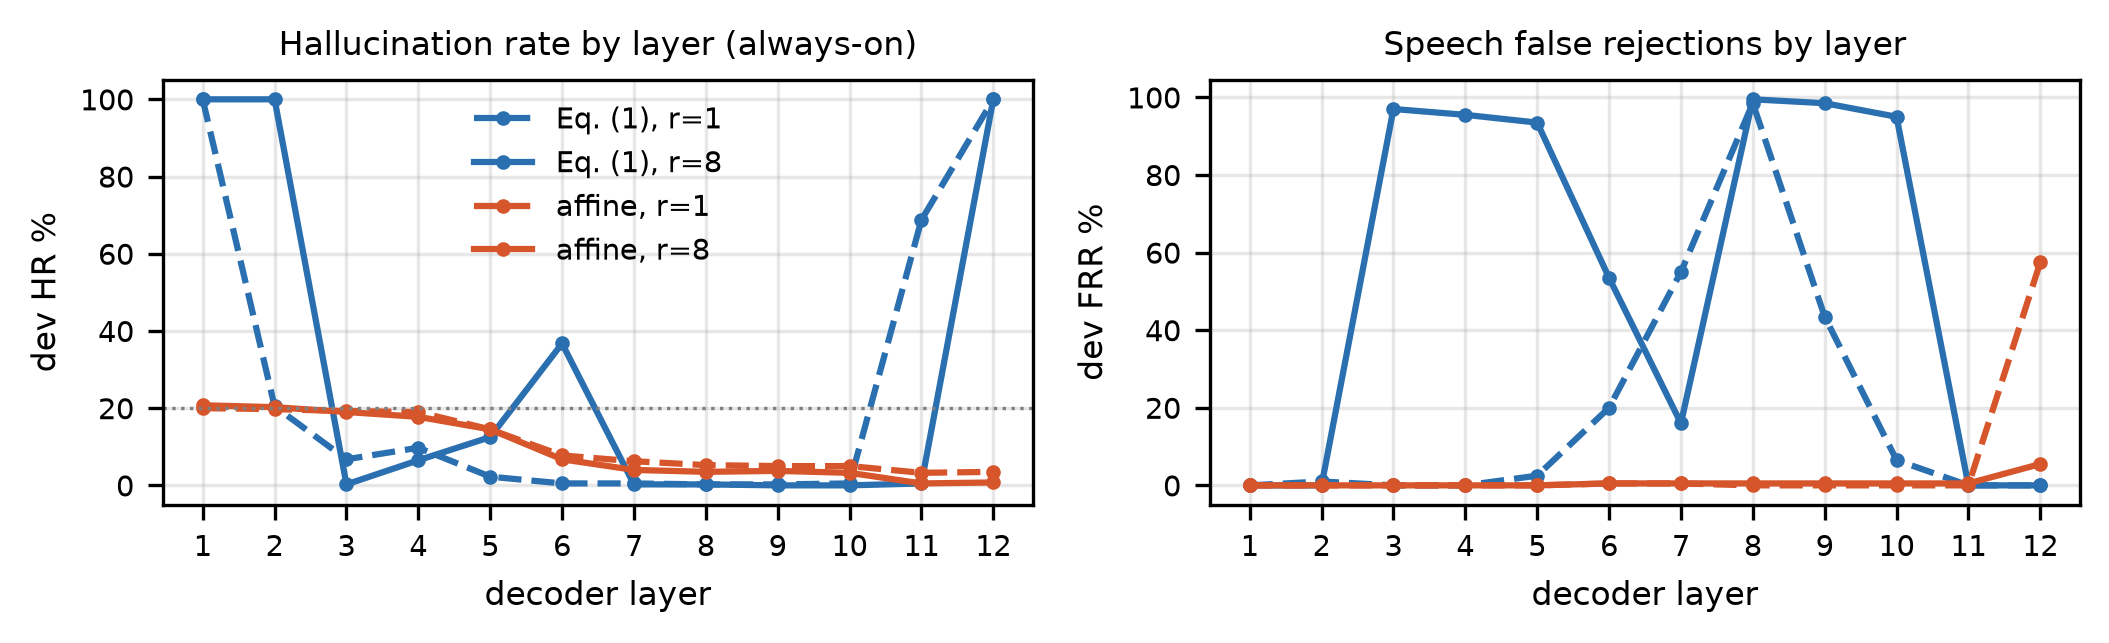
\includegraphics[width=0.9\textwidth]{fig_layers.png}
\caption{Development HR (left) and FRR (right) by decoder layer, always-on, $\alpha = 1$, for Eq.~\eqref{eq:proj} (blue) and the affine Eq.~\eqref{eq:affine} (orange) at ranks 1 and 8. Dotted: plain Whisper.}
\label{fig:layers}
\end{figure*}

\subsection{Affine variant}
\label{sec:affine}
\emph{Held-out results.} The selected affine setting ($\ell$10 $r$2, $\alpha = 1$, $\gamma = 0.05$) keeps almost all speech: FRR is 0.35\% and WER 5.68\%, against 1.35\% and 6.58\% for Eq.~\eqref{eq:proj}. It removes far fewer hallucinations, though: mean HR is 12.61\%, against 4.0\% on development data and 1.27\% for Eq.~\eqref{eq:proj} (Table~\ref{tab:main}). The gap comes mostly from FSD50K (22.85\%), whose sound classes are not in ESC-50; even ESC-50 folds 4--5 reach 8.38\%. The tuned Eq.~\eqref{eq:proj} setting moved much less from dev to test (0.5\% to 1.27\%). At the paper's point the affine edit gives similar numbers (HR 13.50\%, FRR 0.10\%).

\emph{Against the threshold.} $\tau = 0.17$ is better on hallucinations (0.87\% vs.\ 12.61\% HR) but rejects more speech (24 vs.\ 4 utterances, $p = 1.8\cdot10^{-4}$); the WER difference is not significant ($-0.25$ [$-0.55$, 0.03] points). At equal HR ($\tau = 0.46$) the threshold again dominates: it rejects no speech where the affine method rejects 7 (Table~\ref{tab:paired}). In Fig.~\ref{fig:tradeoff} the selected affine points lie above the plotted range, and affine at $\ell$11 $r$8 lies to the right of the threshold curve, like the other projections.

\emph{Why the edit fails at other settings.} The centre $c$ is the mean state at the SOT position, but the hook edits every position. At later positions the states lie far from $c$, so the edit adds a large constant shift. On gated speech at $\ell$11 $r$8 the decoder then emits only language tokens (``\texttt{<|zh|><|zh|>}\ldots''): HR is low (1.37\%), but WER on the edited utterances is 99.6\%, so mean WER is 16.84\% (Table~\ref{tab:main}). This is the 100\% WER at FRR 0\% in Fig.~\ref{fig:stage1}.

\emph{Editing only the SOT position.} The obvious fix is to apply Eq.~\eqref{eq:affine} at the SOT position only, which is also where $c$ is estimated. This fix has a consequence that follows from the architecture alone: the decoder's self-attention is causal, so the SOT state at every layer, and hence $\pns$, depends only on the SOT input and the audio. The edited SOT state, and therefore every gate and rejection decision, is identical whether the edit is applied at one position or at all of them. Only the text of accepted clips can change. For any affine setting, SOT-only editing therefore leaves FRR exactly unchanged and can only lower HR, because an accepted clip can at most turn from non-empty to empty. Applied to the saved per-clip outputs, at $\ell$11 $r$8 this gives an exact FRR of 3.15\% and HR $\le$ 1.37\%. Rejected utterances alone already contribute 2.18 WER points. If the accepted utterances decode as plain Whisper decodes them, mean WER would fall from 16.84\% to about 7.45\% (3.83\% / 11.08\%). This is an estimate, since later positions still attend to the edited SOT state. Either way the setting stays dominated by $\tau = 0.17$ (HR 0.87\%, FRR 1.35\%, WER 5.93\%) on both HR and FRR. At the selected $\ell$10 $r$2 the edit already leaves accepted transcripts intact (WER 5.68\% against 5.66\% under the same estimate), so SOT-only editing would change essentially nothing. Whatever the decoding fix, the projection acts on speech and non-speech only through the rejection decision, which the edit at the SOT position fully determines. Because that decision cannot beat a tuned threshold, no position-wise refinement of the affine edit can either.

\emph{Side effect on speech.} Always-on affine lowers test-clean WER from 3.31\% to 2.92\% (paired bootstrap $-0.39$ [$-0.77$, $-0.09$] points). Most of the gain comes from a few utterances that plain Whisper cut short, and it does not carry over to test-other ($+0.24$ [$-0.17$, 0.69]), so we do not count it as an improvement.

\subsection{Robustness of the basis}
\label{sec:robust}
Two choices in the basis construction, both inherited from~\cite{abbasi2026hsp}, could make the results fragile. Both can be checked offline on the saved SOT states of the 1,200 calibration clips, which store all 12 layers (Table~\ref{tab:robust}).

\emph{Pairing.} The basis construction of Sec.~\ref{sec:subspace} pairs the 256 hallucinated clips with the first 256 empty ones in file order, leaving 688 empty clips unused. We refit $B$ with 20 random pairings (random subsets of $F$, random order) and compare subspaces by the mean squared cosine of their principal angles (1 = identical). The leading direction is stable: from layer 5 on, its overlap with the file-order basis is at least 0.98 for every seed. It is also almost exactly the normalised difference of the two class means, computed from all 1,200 clips (cosine 0.98 to 0.998). Higher directions are not stable. At the selected affine setting ($\ell$10 $r$2) the overlap falls to 0.68 for the worst seed, so that setting partly depends on the arbitrary pairing. A mean-difference direction, or the full class covariances as in closed-form erasure~\cite{belrose2023leace}, would remove this arbitrariness at rank 1.

\emph{Calibration--development overlap.} The 400 development clips are among the 1,200 used to fit $B$ and $c$. We refit both on the 800 calibration clips outside the development set and score the development clips. How well the leading coordinate separates hallucinated from empty development clips barely changes (AUROC 0.945 in-sample vs.\ 0.948 disjoint at $\ell$10; 0.944 vs.\ 0.945 at $\ell$11). The centre $c$ moves by 0.3\% of its norm. The overlap therefore inflates development results little. It does not explain the affine variant's drop from dev to held-out HR, which is largest on FSD50K, whose sound classes are absent from ESC-50. A fully disjoint calibration/development split is nonetheless the correct protocol for future runs.

\begin{table}[!t]
\centering
\caption{Stability of the basis (offline, saved calibration states)}
\label{tab:robust}
\setlength{\tabcolsep}{3pt}
\begin{tabular}{@{}lccccc@{}}
\toprule
& \multicolumn{2}{c}{Random pairing} & & \multicolumn{2}{c}{Dev AUROC, 1st dir.} \\
\cmidrule(lr){2-3}\cmidrule(l){5-6}
Setting & \makecell{Overlap\\mean (min)} & \makecell{Cos.\ to\\mean diff.} & \makecell{Overlap\\disjoint} & \makecell{In-\\sample} & \makecell{Dis-\\joint} \\
\midrule
$\ell$10 $r$1 (paper) & 0.99 (0.98) & 0.99 & 0.98 & 0.945 & 0.948 \\
$\ell$10 $r$2 (affine) & 0.87 (0.68) & 0.99 & 0.89 & 0.945 & 0.948 \\
$\ell$11 $r$8 (Eq.~1) & 0.90 (0.86) & 1.00 & 0.85 & 0.944 & 0.945 \\
$\ell$12 $r$1 & 0.99 (0.98) & 0.98 & 0.99 & 0.916 & 0.918 \\
\bottomrule
\end{tabular}\\[3pt]
\parbox{0.95\columnwidth}{\footnotesize Random pairing: 20 seeds. Overlap: mean squared cosine of the principal angles to the file-order basis (1 = same subspace). Cos.\ to mean diff.: norm of the projection of the normalised class-mean difference onto $\operatorname{span}(B)$. Overlap disjoint: basis fitted without the 400 dev clips. AUROC: leading coordinate (after centring) separating hallucinated from empty dev clips.}
\end{table}

% ---------------------------------------------------------------------------
\section{Discussion}
\label{sec:discussion}

Our results point to eight issues in the evaluation of~\cite{abbasi2026hsp}.
\begin{enumerate}
\item \emph{The key control is missing.} The $\tau$ sweep in~\cite{abbasi2026hsp} stops at 0.5 and is described as changing little, yet its own medium ablation shows plain HR falling from 29.49\% to 13.08\% as $\tau$ goes from 0.6 to 0.4. A threshold chosen by the paper's own rule matches or beats every projection setting we tried.
\item \emph{At the published small setting the edit adds nothing on speech.} Every gated speech utterance is rejected; the gate-open rate on speech and the fate of projected utterances should be reported.
\item \emph{WER mixes two errors.} Counting a rejected utterance as all deletions is correct but hides whether the edit damages transcription. On the same accepted utterances it does not; the cost is rejection only. The paper's own numbers imply a rejected-word share of 0.32 to 0.88 times FRR, i.e., short utterances are rejected.
\item \emph{Projection to zero is not neutral} (Sec.~\ref{sec:lastlayer}). An affine target, the principled choice~\cite{belrose2023leace}, fixes the last layer, but a single centre applied at every position creates new failures (Sec.~\ref{sec:affine}).
\item \emph{Calibration labels are defined by $\pns$}, so the subspace partly re-learns the no-speech read-out, consistent with unchanged AUROC.
\item \emph{Tuning ignores noisy speech.} Our Eq.~\eqref{eq:proj} setting had 0\% FRR on dev-clean but 2.5--3.3\% on test-other.
\item \emph{Internal inconsistencies.} The validation WER in Fig.~1 and Sec.~5.1 of~\cite{abbasi2026hsp} differ (3.94\% vs.\ 11.59\%); the medium $\alpha$ is given as 0.75 and 1.0; the FSD50K plain HR is identical (21.35\%) for small and large-v3; Table~5 at $\tau = 0.6$ disagrees with Table~1 for medium (plain HR 29.49\% vs.\ 27.66\%, projected 5.09\% vs.\ 4.06\%); the FSD50K count fits removing speech but not music; and Calm-Whisper is compared under a different HR definition.
\item \emph{Development clips are calibration clips.} Parameters are selected on non-speech clips that also fit the basis. We inherited this protocol; on Whisper small its effect on the basis is small (Sec.~\ref{sec:robust}), but it should be avoided.
\end{enumerate}

Wilson intervals on the paper's own large-v3 rates also qualify one claim: WhisperX VAD beats gated projection on ESC-50 (4.13\% [2.96, 5.74] vs.\ 8.38\% [6.65, 10.50]), ties on UrbanSound8K, and loses only on FSD50K (8.55\% vs.\ 1.15\%).

% ---------------------------------------------------------------------------
\section{Limitations}

We test Whisper small only, with one seed and held-out subsets of 1,000--2,000 clips per set; medium and large-v3, where~\cite{abbasi2026hsp} reports its largest gains, need a larger GPU. Development data are small (400 non-speech and 200 speech clips), so dev HR moves in steps of 0.25\% and several thresholds tie. The WER of SOT-only affine editing is an estimate from saved outputs, and the robustness checks of Sec.~\ref{sec:robust} are made on the basis, not by re-decoding; its FRR and HR bound are exact. We did not run the WhisperX VAD baseline. fp16 results depend slightly on batch size, which we kept fixed at 16.

% ---------------------------------------------------------------------------
\section{Conclusion}

Gated hallucination space projection reproduces on Whisper small: it removes most non-speech hallucinations, our rates at the paper's setting are within about a point of the published ones, and the edit does not harm the transcripts it keeps. Its benefit, however, comes from Whisper's own no-speech probability. Lowering the rejection threshold, chosen on development data by the same rule, does at least as well with no change to the model, and at the paper's operating point the method is that threshold. Moving states to the empty-class mean instead of zero fixes the last-layer failure and nearly removes false rejections, but its single SOT-position centre breaks decoding at many settings. Its selected setting also generalises poorly to held-out sounds, so it does not beat the threshold either. Restricting the edit to the SOT position repairs the transcripts but, because the decoder is causal, leaves every rejection unchanged, so it cannot change this conclusion. Before projection can be called an improvement, the comparison against a tuned threshold should be repeated on medium and large-v3.

% ---------------------------------------------------------------------------
\section*{Code and Data Availability}

The notebook, all saved per-clip results and the interactive dashboard are publicly available at \repo. The dashboard is a local web page that runs a curated test clip, a microphone recording or an audio file through five methods at once (plain Whisper at $\tau = 0.6$ and 0.17, both gated projection settings, and the gated affine variant). It shows the log-Mel input and, per method, $\pns$ before and after the edit against $\gamma$ and $\tau$, the verdict and the output, with a word diff against the reference for speech. On twelve curated clips its live decisions match the saved run in all 60 cases.

\section*{Author Contributions}

Nongmaithem Hans researched the topic, selected the reference paper and executed all experimental runs (calibration, hyperparameter sweeps and held-out evaluations) on a 6\,GB laptop GPU. Hans engineered the memory and runtime optimisations: fp16 execution, a shared encoder pass, skipping decodes that are rejected anyway, and checkpointing with resume. Hans designed and carried out the extended analyses: the reproduction comparisons, the tuned threshold baseline, the paired McNemar and bootstrap significance tests, the gate and last-layer mechanics analyses, and the affine projection variant. Hans designed the interactive dashboard and implemented its live inference server, and prepared the presentation slides.

Ravikant Sharma built the dataset ingestion, preprocessing and label-filtering pipeline across ESC-50, UrbanSound8K, FSD50K and LibriSpeech, and wrote the initial notebook implementation covering Whisper decoding, forward-hook registration, SVD subspace estimation, and the HR, WER and FRR metrics. Ravikant audited the methodological and numerical inconsistencies in the reference paper (Sec.~\ref{sec:discussion}), synthesised the experimental outputs and authored the manuscript. For the dashboard, Ravikant curated the twelve demonstration clips from the evaluation outputs, built the waveform, spectrogram and word-diff views, and verified the live results against the saved run.

Both authors discussed the experimental findings and reviewed the final report.

\emph{Use of AI tools.} We used AI assistance in a limited set of places. During the training and evaluation runs, an AI assistant helped us locate and fix bugs in our code. AI assistance was also used in building the interactive dashboard. The presentation slides were made by hand; the animated HTML version of the presentation was adapted with AI assistance. AI assistance was also used for the follow-up analyses in Sec.~\ref{sec:affine} (SOT-only editing) and Sec.~\ref{sec:robust}, which are computed from our saved calibration states and per-clip outputs, and for typesetting this report. Apart from these follow-up analyses, the research design, experiments, analysis and conclusions are the authors' own. We reviewed all AI-assisted code and material, and we take full responsibility for the content of this report.

\section*{Acknowledgment}

This work was carried out as the course project for AI553 Speech and Audio Processing at the Indian Institute of Technology Ropar. We thank the instructors, Dr.\ Anusha Prakash and Dr.\ Arun Kumar Sharma, for their guidance.

% ---------------------------------------------------------------------------
\begin{thebibliography}{11}

\bibitem{abbasi2026hsp}
M.~Abbasihafshejani and M.~Jadliwala, ``Reducing hallucinated transcripts in Whisper via hallucination space projection,'' \emph{arXiv preprint arXiv:2609.04561}, 2026.

\bibitem{radford2023whisper}
A.~Radford, J.~W. Kim, T.~Xu, G.~Brockman, C.~McLeavey, and I.~Sutskever, ``Robust speech recognition via large-scale weak supervision,'' in \emph{Proc. Int. Conf. Mach. Learn. (ICML)}, 2023.

\bibitem{baranski2025boh}
M.~Bara\'nski \emph{et al.}, ``Investigation of Whisper ASR hallucinations induced by non-speech audio,'' in \emph{Proc. IEEE Int. Conf. Acoust., Speech, Signal Process. (ICASSP)}, 2025.

\bibitem{wang2025calm}
Y.~Wang \emph{et al.}, ``Calm-Whisper: Reduce Whisper hallucination on non-speech by calming crazy heads down,'' in \emph{Proc. Interspeech}, 2025.

\bibitem{bain2023whisperx}
M.~Bain, J.~Huh, T.~Han, and A.~Zisserman, ``WhisperX: Time-accurate speech transcription of long-form audio,'' in \emph{Proc. Interspeech}, 2023.

\bibitem{belrose2023leace}
N.~Belrose \emph{et al.}, ``LEACE: Perfect linear concept erasure in closed form,'' in \emph{Proc. Adv. Neural Inf. Process. Syst. (NeurIPS)}, 2023.

\bibitem{piczak2015esc}
K.~J. Piczak, ``ESC: Dataset for environmental sound classification,'' in \emph{Proc. ACM Int. Conf. Multimedia}, 2015.

\bibitem{salamon2014urbansound}
J.~Salamon, C.~Jacoby, and J.~P. Bello, ``A dataset and taxonomy for urban sound research,'' in \emph{Proc. ACM Int. Conf. Multimedia}, 2014.

\bibitem{fonseca2022fsd50k}
E.~Fonseca, X.~Favory, J.~Pons, F.~Font, and X.~Serra, ``FSD50K: An open dataset of human-labeled sound events,'' \emph{IEEE/ACM Trans. Audio, Speech, Lang. Process.}, vol.~30, 2022.

\bibitem{panayotov2015librispeech}
V.~Panayotov, G.~Chen, D.~Povey, and S.~Khudanpur, ``LibriSpeech: An ASR corpus based on public domain audio books,'' in \emph{Proc. IEEE Int. Conf. Acoust., Speech, Signal Process. (ICASSP)}, 2015.

\bibitem{mcnemar1947}
Q.~McNemar, ``Note on the sampling error of the difference between correlated proportions or percentages,'' \emph{Psychometrika}, vol.~12, no.~2, 1947.

\end{thebibliography}

\end{document}
